\documentclass[conference]{IEEEtran}
\usepackage{graphicx}
\usepackage{amsmath}
\usepackage{hyperref}
\usepackage{listings}
\usepackage{color}
\usepackage{float}
\usepackage{caption}
\usepackage{subcaption}

\title{Hệ Thống Quản Lý Giao Thông Thông Minh: Giải Pháp Dựa Trên Trí Tuệ Nhân Tạo Cho Tối Ưu Hóa Giao Thông Đô Thị}

\author{
    \IEEEauthorblockN{Tên Tác Giả}
    \IEEEauthorblockA{Khoa Công Nghệ Thông Tin\\
    Tên Trường Đại Học\\
    Email: tacgia@example.com}
}

\begin{document}

\maketitle

\begin{abstract}
Tắc nghẽn giao thông đô thị là một thách thức nghiêm trọng ảnh hưởng đến chất lượng cuộc sống và hiệu quả kinh tế. Bài báo trình bày thiết kế và triển khai Hệ Thống Quản Lý Giao Thông Thông Minh, sử dụng các kỹ thuật trí tuệ nhân tạo tiên tiến và phân tích dữ liệu thời gian thực để tối ưu hóa luồng giao thông đô thị. Hệ thống tích hợp nhiều nguồn dữ liệu như camera giám sát, cảm biến IoT, thiết bị GPS và ứng dụng di động để cung cấp điều khiển tín hiệu giao thông thông minh, dự đoán tắc nghẽn và tối ưu hóa lộ trình. Bài báo mô tả kiến trúc hệ thống, các thuật toán cốt lõi và quá trình triển khai, chứng minh hiệu quả của giải pháp trong việc cải thiện lưu thông đô thị.
\end{abstract}

\begin{IEEEkeywords}
Quản lý giao thông thông minh, Trí tuệ nhân tạo, Tối ưu hóa tín hiệu giao thông, Dự đoán tắc nghẽn, Tối ưu hóa lộ trình, Phân tích thời gian thực
\end{IEEEkeywords}

\section{Giới thiệu}
Sự gia tăng dân số và đô thị hóa đã dẫn đến tình trạng tắc nghẽn giao thông nghiêm trọng tại nhiều thành phố lớn, gây ra thời gian di chuyển kéo dài, ô nhiễm môi trường và tổn thất kinh tế. Các hệ thống quản lý giao thông truyền thống thường dựa trên các chu kỳ tín hiệu cố định và dữ liệu hạn chế, dẫn đến hiệu quả thấp trong việc điều phối lưu lượng. Hệ Thống Quản Lý Giao Thông Thông Minh được đề xuất nhằm cách mạng hóa việc điều khiển giao thông đô thị thông qua việc ứng dụng các kỹ thuật trí tuệ nhân tạo và phân tích dữ liệu thời gian thực. Hệ thống xử lý dữ liệu đa nguồn để điều chỉnh linh hoạt tín hiệu giao thông, dự đoán tắc nghẽn và đề xuất lộ trình tối ưu, từ đó giảm thiểu thời gian chờ và khí thải.

\section{Tổng quan hệ thống}
Kiến trúc hệ thống bao gồm ba thành phần chính: thu thập dữ liệu, xử lý AI và ứng dụng người dùng. Dữ liệu được thu thập từ camera giám sát, cảm biến IoT, thiết bị GPS và ứng dụng di động, được đưa vào pipeline xử lý để lưu trữ và phân tích. Các mô-đun AI thực hiện dự đoán lưu lượng, tối ưu hóa tín hiệu và lập kế hoạch lộ trình. Giao diện người dùng bao gồm bảng điều khiển tương tác xây dựng trên nền tảng Streamlit, cung cấp khả năng giám sát và điều khiển thời gian thực.

\begin{figure}[H]
    \centering
    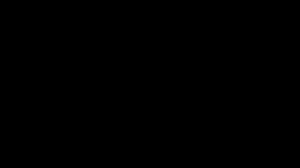
\includegraphics[width=0.48\textwidth]{imgs/images.png}
    \caption{Tổng quan kiến trúc hệ thống}
    \label{fig:architecture_vn}
\end{figure}

\section{Phương pháp luận}
\subsection{Nguồn dữ liệu và xử lý}
Hệ thống tích hợp các luồng dữ liệu đa dạng, bao gồm video từ camera giám sát, dữ liệu cảm biến, và dữ liệu GPS. Quá trình tiền xử lý dữ liệu bao gồm làm sạch, chuẩn hóa và trích xuất đặc trưng để chuẩn bị cho các mô hình AI.

\subsection{Tối ưu hóa tín hiệu giao thông}
Thuật toán di truyền được sử dụng để tối ưu hóa thời gian xanh của tín hiệu giao thông cho bốn hướng (bắc, nam, tây, đông). Hàm fitness mô hình hóa độ trễ dựa trên phân bổ thời gian xanh và lưu lượng xe. Thuật toán tiến hóa qua các thế hệ để tìm ra cấu hình tín hiệu tối ưu, thích ứng với điều kiện giao thông thời gian thực được phát hiện qua phân tích video.

\subsection{Phân tích video giao thông}
Phát hiện và theo dõi phương tiện được thực hiện bằng mô hình học sâu YOLO kết hợp với DeepSort để theo dõi đa đối tượng. Hệ thống tính toán vận tốc, hướng di chuyển và đếm số lượng xe trong vùng quan tâm (ROI). Mức độ tắc nghẽn được suy ra từ mật độ và lưu lượng xe, hỗ trợ điều khiển tín hiệu thích ứng và cảnh báo.

\subsection{Tối ưu hóa lộ trình và dự đoán tắc nghẽn}
Dữ liệu lịch sử và thời gian thực được sử dụng để xây dựng đồ thị trọng số biểu diễn mạng lưới đường bộ đô thị. Trọng số bao gồm khoảng cách, báo cáo tai nạn và cường độ giao thông. Thuật toán Dijkstra tính toán đường đi ngắn nhất, trong khi dự đoán tắc nghẽn và thời gian di chuyển được tạo ra dựa trên các quy tắc và trực quan hóa qua bản đồ tương tác.

\section{Triển khai}
Hệ thống được triển khai chủ yếu bằng Python, sử dụng các framework và thư viện như Streamlit cho bảng điều khiển, Flask cho API backend, PyTorch cho học sâu, OpenCV cho xử lý video và Folium cho trực quan bản đồ. Dịch vụ backend xử lý video giao thông tải lên, đếm xe và chạy thuật toán di truyền để tối ưu tín hiệu.

\subsection{Bảng điều khiển}
Bảng điều khiển xây dựng trên Streamlit cung cấp ba module chính: Phân tích video giao thông, Tối ưu hóa lộ trình và Mô phỏng tín hiệu. Người dùng có thể xem phân tích video thời gian thực, chọn lộ trình để dự đoán tắc nghẽn và mô phỏng điều khiển tín hiệu với thời gian xanh thích ứng.

\subsection{Dịch vụ backend}
API Flask nhận video tải lên, thực hiện phát hiện xe bằng YOLOv4 và tối ưu tín hiệu giao thông qua thuật toán di truyền. Thiết kế mô-đun giúp hệ thống dễ dàng mở rộng và tích hợp với các hệ thống thành phố thông minh khác.

\section{Kết quả và thảo luận}
Hệ thống thể hiện khả năng giám sát giao thông thời gian thực và điều khiển tín hiệu thích ứng hiệu quả. Thuật toán di truyền hội tụ đến các cấu hình thời gian xanh tối ưu, giảm thiểu tổng độ trễ. Phân tích video chính xác trong việc phát hiện và theo dõi phương tiện, cung cấp số liệu tắc nghẽn đáng tin cậy. Tối ưu hóa lộ trình hỗ trợ người lái tránh khu vực tắc nghẽn, cải thiện thời gian di chuyển.

\section{Kết luận}
Hệ Thống Quản Lý Giao Thông Thông Minh chứng minh tiềm năng của trí tuệ nhân tạo và phân tích thời gian thực trong việc cải thiện điều khiển giao thông đô thị. Công việc tương lai bao gồm tích hợp dữ liệu trực tiếp, nâng cao mô hình học máy để tăng độ chính xác dự đoán và mở rộng tùy chỉnh người dùng.

\section*{Lời cảm ơn}
Chúng tôi xin cảm ơn cộng đồng mã nguồn mở và các cộng tác viên đã cung cấp các công cụ và hỗ trợ quý giá cho dự án này.

\bibliographystyle{IEEEtran}
\bibliography{references}

\end{document}
